\documentclass[11pt,a4paper]{article}
\usepackage{listings}
\usepackage[utf8]{inputenc}
\usepackage{mathtools}
\usepackage[norsk]{babel}
\usepackage{graphicx}
\usepackage{gensymb}
\usepackage{wasysym}
\usepackage{hyperref}
\usepackage{setspace}
\usepackage{tikz}
\usepackage{amsthm}
\usepackage{amsmath}
\usepackage{mathrsfs}
\usepackage{amssymb}
\usepackage{color}
\usepackage{rotating}
\usepackage{pgfplots}


\usetikzlibrary{arrows}
\usetikzlibrary{shapes, automata}


\newcommand{\intt}{integritetsregler}
\newcommand{\inttt}{integritetsregel}
\newcommand{\Intt}{Integritetsregler}
 
\definecolor{dkgreen}{rgb}{0,0.6,0}
\definecolor{gray}{rgb}{0.5,0.5,0.5}
\definecolor{mauve}{rgb}{0.58,0,0.82}


\lstset{ %
  language=Java,                % the language of the code
  basicstyle=\small,           % the size of the fonts that are used for the code
  numbers=left,                   % where to put the line-numbers
  numberstyle=\small\color{gray},  % the style that is used for the line-numbers
  stepnumber=1,                   % the step between two line-numbers. If it's 1, each line 
                                  % will be numbered
  numbersep=5pt,                  % how far the line-numbers are from the code
  backgroundcolor=\color{white},      % choose the background color. You must add \usepackage{color}
  showspaces=false,               % show spaces adding particular underscores
  showstringspaces=false,         % underline spaces within strings
  showtabs=false,                 % show tabs within strings adding particular underscores
  frame=none,                   % adds a frame around the code
  rulecolor=\color{black},        % if not set, the frame-color may be changed on line-breaks within not-black text (e.g. commens (green here))
  tabsize=2,                      % sets default tabsize to 2 spaces
  captionpos=b,                   % sets the caption-position to bottom
  breaklines=true,                % sets automatic line breaking
  breakatwhitespace=false,        % sets if automatic breaks should only happen at whitespace
  title=\lstname,                   % show the filename of files included with \lstinputlisting;
                                  % also try caption instead of title
  keywordstyle=\color{blue},          % keyword style
  commentstyle=\color{dkgreen},       % comment style
  stringstyle=\color{mauve},         % string literal style
  escapeinside={\%*}{*)},            % if you want to add LaTeX within your code
  morekeywords={*,...}               % if you want to add more keywords to the set
}

\setlength{\parskip}{5mm}

\newtheoremstyle{mytheoremstyle} 	% name
    {\topsep}                    			% Space above
    {\topsep}                    			% Space below
    {\itshape}                   			% Body font
    {}                           			% Indent amount
    {\scshape}                   			% Theorem head font
    {.}                          			% Punctuation after theorem head
    {.5em}                       			% Space after theorem head
    {} 				 			% Theorem head spec (can be left empty, meaning ‘normal’)

\title{Notater: INF2220}
\author{Veronika Heimsbakk \\ 
veronahe@student.matnat.uio.no}
\begin{document}

\maketitle{}
\tableofcontents
\newpage{}

\section*{Introduksjon}
Dette er notater til kurset INF2220--Algoritmer og datastrukturer ved Universitetet i Oslo. Disse notatene er i all hovedsak basert på forelesningsfoiler, egne notater og læreboka. Brukes til repetisjon før eksamen og som notater under eksamen. Merk at notatene helt sikkert inneholder feil og mangler.


%%% KJØRETID %%%
\section{Kjøretid}
Ettersom kjøretiden til algoritmer som regel er et veldig komplekst uttrykk, så holder det at denne estimeres. Denne typen estimering kalles \textbf{asymptotic analysis}, eller \textbf{big-O} notasjon.

\theoremstyle{mytheoremstyle}
\newtheorem{onotasjon}{Definisjon}[section]
\begin{onotasjon}
La $f$ og $g$ være funksjoner $f,g: \mathcal{N} \rightarrow \mathcal{R}^+$. Sier at $\textbf{f(n) = O(g(n))}$ hvis det eksisterer positive heltall $c$ og $n_0$ slik at for hvert heltall $n \geq n_0$,
$$f(n) \leq c g(n).$$
Når $f(n) = O(g(n))$, sier vi at $g(n)$ er \textbf{upper bound} for $f(n)$, eller mer presist at $g(n)$ er \textbf{asymptotic upper bound} for $f(n)$.
\end{onotasjon}

\begin{table}[h!]
\centering
\begin{tabular}{rl}
\textbf{Funksjon}&\textbf{Navn}\\
$1$&Konstant\\
$\log n$&Logaritmisk\\
$n$&Lineær\\
$n \log n$&\\
$n^2$&Kvadratisk\\
$n^3$&Kubisk\\
$2^n$&Eksponensiell\\
$n!$&\\
\end{tabular}
\label{tab:ofunc}
\caption{Vanlige funksjoner for O$(n)$}
\end{table}

\begin{figure}[h!]
\centering
\begin{tikzpicture}
\draw[thick, ->] (0,0) -- (5,0) node[below] {Input size  (N)};
\draw[thick, ->] (0,0) -- (0,5) node[left] {Running time};

\foreach \x in {1,2,3,4}
	\draw (\x cm, 2pt) -- (\x cm, -2pt);
\foreach \y in {1,2,3,4}
	\draw (2pt, \y cm) -- (-2pt, \y cm);

\draw[red, domain=0:2.2] plot (\x, {\x^2}) node[right]{$n^2$};
\draw[blue, domain=0:3.5] plot (\x, {\x}) node[right] {$n$};
\draw[black, domain=0:1.7] plot (\x, {\x^3}) node[right] {$n^3$};
\end{tikzpicture}
\label{fig:ofunc}
\caption{Noen funksjoner for O$(n)$.}
\end{figure}

Et eksempel på enkel beregning av kjøretid for kode er:
\begin{lstlisting}
// O(n)
for (i = 0; i < n; i++)
	array[i] = 0;

// O(n^2)
for (i = 0; i < n; i++)
	for (j = 0; j < n; j++)
		array[i][j] = 0;
\end{lstlisting}


%%% TRÆR %%%
\section{Trær}
\newtheorem{tre}{Definisjon}[section]
\begin{tre}
Et \textbf{tre} er en samling \textbf{noder}. Et ikke-tomt tre består av en \textbf{rot}-node, og null eller flere ikke-tomme \textbf{subtrær}. Fra roten går en \textbf{rettet kant} til roten i hvert subtre.
\end{tre}

\begin{figure}[h!]
\centering
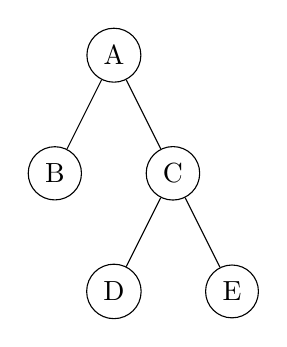
\begin{tikzpicture}[every node/.style={circle, draw=black}]
\node{A}
	child {node {B}}
	child {node {C}
		child {node {D}}
		child {node {E}}
	}
;
\end{tikzpicture}
\label{fig:basictree}
\caption{Eksempel på et tre.}
\end{figure}

I figur \ref{fig:basictree}, så er A rot-noden. B og C er barna til A, og C er forelder til løvnodene D og E.

% Traversering
\subsection{Traversering}
\begin{description}
\item[Pre-order] rot, venstre barn, høyre barn
\item[In-order] venstre barn, rot, høyre barn
\item[Post-order] venstre barn, høyre barn, rot
\end{description}

\begin{lstlisting}
/* IN-ORDER TRAVERSAL */

public void inOrder (Node node) {
	if (node != null) {
		inOrder(node.left);
		// do something with the node
		inOrder(node.right);
	}
}

/* PRE-ORDER TRAVERSAL */

public void preOrder (Node node) {
	if (node != null) {
		// do something with the node
		preOrder(node.left);
		preOrder(node.right);
	}
}

/* POST-ORDER TRAVERSAL */

public void postOrder (Node node) {
	if (node != null) {
		postOrder(node.left);
		postOrder(node.right);
		// do something with the node
	}
}
\end{lstlisting}

% Terminologi
\subsection{Terminologi}
\begin{description}
\item[Vei] Eller en \textit{sti} fra node $n_1$ til $n_k$ er definert som en sekvens $n_1, n_2, \dots, n_k$, slik at $n_i$ er forelder til $n_{i+1}$ for $1 \leq i \leq k$.
\item[Lengden] Lengden av veien er antall \textit{kanter} på veien; $k-1$.
\item[Dybde] Definert av den unike veien fra roten til noden. Rotens dybde er 0.
\item[Høyden] Definert som lengden av den \textit{lengste} veien fra noden til en løvnode. Alle løvnoder har høyde 0. Høyden til et tre er lik høyden til roten.
\end{description}


%%% BINÆRTRÆR %%%
\subsection{Binærtrær}
I et binærtre er et tre der hver node aldri har mer enn to barn. I INF2220 er fokuset på \textit{binære søketrær}. For binære søketrær skal følgende holde for hver node i treet:
\begin{itemize}
\item
Alle verdiene i \textit{venstre} subtre er \textit{mindre} enn verdien i noden selv.
\item
Alle verdiene i \textit{høyre} subtre er \textit{større} enn verdien i noden selv.
\end{itemize}

\begin{figure}[h!]
\centering
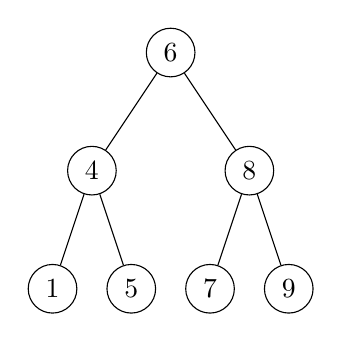
\begin{tikzpicture}[every node/.style={circle, draw=black}, 
				   level 1/.style={sibling distance=20mm},
				   level 2/.style={sibling distance=10mm}]
\node{6}
	child {node {4}
		child {node {1}}
		child {node {5}}
	}
	child {node {8}
		child {node {7}}
		child {node {9}}
	}
;
\end{tikzpicture}
\label{fig:simplebst}
\caption{Eksempel på et binært søketre.}
\end{figure}

\subsection{Rød-svarte trær}
Et rød-svart tre er et binært søketre der hver node er farget enten rød eller svart slik at følgende holder:
\begin{enumerate}
\item
Roten er svart.
\item
Hvis en node er rød, så må barna være svarte.
\item
Enhver sti fra en node til en null-peker må inneholde samme antall svarte noder.
\end{enumerate}
Dette sikrer at høyden på et slikt tre er maks $2\times\log_2(N+1)$.

\tikzset{
	treenode/.style = {align=center, inner sep=0pt},
	% Sorte noder
	node_black/.style = {treenode, circle, white,
						font=\bfseries, draw=black,
						fill=black, text width=0.8cm},
	% Røde noder
	node_red/.style = {treenode, circle, red, draw=red,
						text width=0.8cm, very thick},
	% Null-pekere
	node_null/.style = {treenode, rectangle, draw=black,
						minimum width=0.3cm, minimum height=0.3cm}
}

\begin{figure}[h!]
\centering
\begin{tabular}{p{4cm}p{4cm}p{4cm}}
1&2&3\\
\begin{tikzpicture}[level 1/.style={sibling distance=20mm},
				   level 2/.style={sibling distance=10mm}]
\node[node_black]{41}
	child {node[node_red] {38}}
	child {node [node_null] {}}
;
\end{tikzpicture}
&
\begin{tikzpicture}[level 1/.style={sibling distance=20mm},
				   level 2/.style={sibling distance=10mm}]
\node[node_black]{38}
	child {node[node_red] {31}}
	child {node [node_red] {41}}
;
\end{tikzpicture}
&
\begin{tikzpicture}[level 1/.style={sibling distance=20mm},
				   level 2/.style={sibling distance=10mm}]
\node[node_black]{38}
	child {node[node_black] {31}
		child {node[node_null] {}}
		child {node[node_red] {12}}
	}
	child {node [node_black] {41}}
;
\end{tikzpicture}\\
Setter inn 41 og 38 etter reglene. 
& Når 31 nå kommer inn, så må vi snu på treet og farge om 38 og 41. 
& Siden løvnodene var røde når 12 skal inn, så må 31 og 41 farges om. 41 skal farges iht. regel nr. 3.\\
\begin{tikzpicture}[level 1/.style={sibling distance=20mm},
				   level 2/.style={sibling distance=10mm}]
\draw[black] (0,1) node[above]{4.};
\node[node_black]{38}
	child {node[node_red] {19}
		child {node[node_black] {12}}
		child {node[node_black] {31}}
	}
	child {node [node_black] {41}}
;
\end{tikzpicture}
&
\begin{tikzpicture}[level 1/.style={sibling distance=20mm},
				   level 2/.style={sibling distance=10mm}]
\draw[black] (0,1) node[above]{5.};
\node[node_black]{38}
	child {node[node_red] {19}
		child {node[node_black] {12}
			child{node[node_red] {8}}
			child{node[node_null] {}}
		}
		child {node[node_red] {31}}
	}
	child {node [node_black] {41}}
;
\end{tikzpicture}
&\\
Når 19 nå kommer inn, så må vi igjen snu på treet for å opprettholde reglene til et BST. Farger nodene på nytt iht. reglene for rød-svarte trær.
&
Til slutt setter vi inn 8 som løvnode til 12. Her trenger vi ikke å snu eller fargelegge.
\end{tabular}
\label{fig:rseks}
\caption{Eksempel på innsetting av tallene 41, 38, 31, 12, 19 og 8 i et rød-svart tre.}
\end{figure}

%%% B-TRÆR %%%
\subsection{B-trær}

%%% MAPS %%%
\section{Maps}

%%% HASHING %%%
\section{Hashing}
Idéen i hashing er å lagre alle elementene i en array (hashtabell) og la verdien i elementet $x$ bestemme indeksen til $x$ i hashtabellen. Egenskaper til en god hash-funksjon er at den er rask å beregne, kan gi alle mulige verdier fra 0 til tabellens størrelse $-1$. Og den git en god fordeling utover tabellindeksene. En hashtabell tilbyr innsetting, sletting og søking med konstant tid.

\subsection{Hash-funksjoner}
\paragraph{Eksempel} med heltall som nøkkel, begrenset antall tabellindekser. La hashfunksjonen være \texttt{hash(x, taleSize) = x mod tableSize}. Husk at hvis \texttt{tableSize} er 10 og alle nøklene slutter på 0, vil alle elementene havne på samme indeks. Huskeregel for dette: la alltid tabellstørrelsen være et primtall. Funksjonen under summerer verdiene til hver bokstav. Dette er en dårlig fordeling dersom tabellstørrelsen er stor.
\begin{lstlisting}
int hash (String key, int tableSize) {
	int hashValue = 0;
	for (i = 0; i < key.length(); i++) 
		hashValue+= key.charAt(i);
	return (hashValue % tableSize);
}
\end{lstlisting}

\subsection{Forskjellige typer hash-tabeller}
\begin{itemize}
\item
\textbf{Seprate chaining} er en hash-tabell hvor hver indeks peker til en liste av elementer.
\item
\textbf{Probing} er rommet mellom hver indeks.
\begin{itemize}
\item
\textit{Lineær probing}; intervallene er satt (normalt 1).
\item
\textit{Kvadratisk probing}; intervallene øker med å legge til et kvadratisk polynom ved startverdi gitt av hashberegningen.
\item
\textit{Dobbel hashing}; intervallene er gitt av en annen hash-funksjon.
\end{itemize}
\end{itemize}

\begin{table}[h!]
\centering
\begin{tabular}{c|c|c|c}
Index & Linear probing & Quadratic probing & Separate chaining\\
\hline
0 & 9679 & 9679 &\\
1 & 4371 & 4371 & \\
2 & 1989 & &\\
3 & 1323 & 1323 & 1323 $\rightarrow$ 6173\\
4 & 6173 & 6173 & 4344\\
5 & 4344 & 4344 &\\
6 & & &\\
7 & & &\\
8 & & 1989 &\\
9 & 4199 & 4199 & 4199 $\rightarrow$ 9679 $\rightarrow$ 1989\\
\end{tabular}
\label{tab:hash}
\caption{Eksempel på hashing.}
\end{table}
I tabell \ref{tab:hash} har vi forskjellige hash-tabeller på tallene \{4371, 1323, 4199, 4344, 9679, 1989\} som skal settes inn i en tabell på størrelse 10, og med hash-funksjon \texttt{H(X) = X mod 10}.

\paragraph{Lineær probing} her tar man tallet og setter inn i hash-funksjonen. Så for første tall (4371) vil indeksen bli 1. Hvis indeksen er opptatt, så plusser man på 1.

\paragraph{Kvadratisk probing} er så og si det samme, men i stedet for å legge til 1 hvis indeksen er opptatt, så legger man på $1^2, 2^2, 3^2,\dots$

\paragraph{Dobbel probing} her lager vi en ny hash-funksjon når indeksen krasjer. Da tar man et tall $P$, som er det største primtallet som er mindre enn tabellstørrelsen. Dette brukes til å lage en ny hash-funksjon \texttt{H(X) = R - (X mod R)}.

\paragraph{Separate chaining} her legges det nye tallet på i en liste om indeksen er opptatt fra før.






\section{Prioritetskø}
\section{Heap}

Skal gjøre operasjonen \texttt{deleteMin()} på følgende heap $\times 3$.

\begin{center}
\scalebox{0.8}{
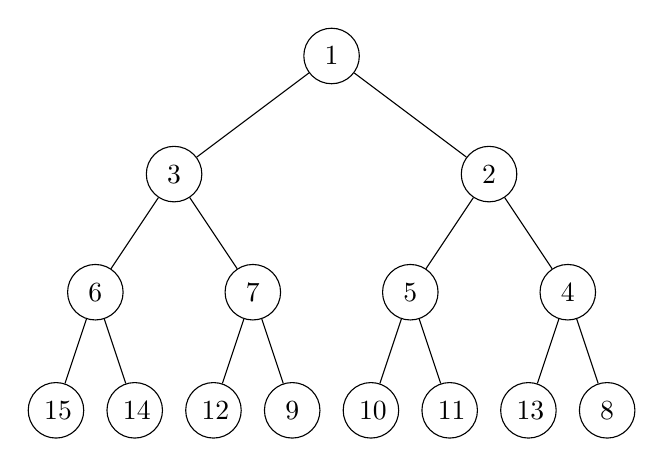
\begin{tikzpicture}[every node/.style={circle, draw=black, text width=0.3cm, align=center},
				   level 1/.style={sibling distance=40mm},
				   level 2/.style={sibling distance=20mm},
				   level 3/.style={sibling distance=10mm}]
\node{1}
	child {node {3}
		child {node {6}
			child {node {15}}
			child {node {14}}
		}
		child {node {7}
			child {node {12}}
			child {node {9}}
		}
	}
	child {node {2}
		child {node {5}
			child {node {10}}
			child {node {11}}
		}
		child {node {4}
			child {node {13}}
			child {node {8}}
		}
	}
;
\end{tikzpicture}
}
\end{center}

Begynner med å slette rot noden 1. Og flytter siste element (8) opp til rot posisjon.

\begin{center}
\scalebox{0.8}{
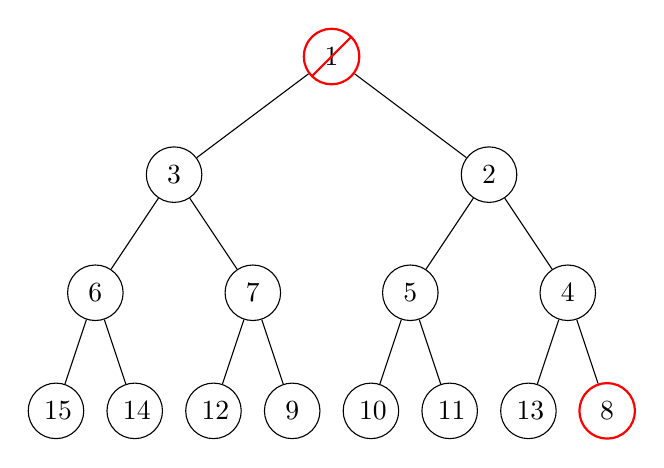
\begin{tikzpicture}[every node/.style={circle, draw=black, text width=0.3cm, align=center},
				   level 1/.style={sibling distance=40mm},
				   level 2/.style={sibling distance=20mm},
				   level 3/.style={sibling distance=10mm}]
\node[draw=red, thick, forbidden sign]{1}
	child {node {3}
		child {node {6}
			child {node {15}}
			child {node {14}}
		}
		child {node {7}
			child {node {12}}
			child {node {9}}
		}
	}
	child {node {2}
		child {node {5}
			child {node {10}}
			child {node {11}}
		}
		child {node {4}
			child {node {13}}
			child {node[draw=red, thick] {8}}
		}
	}
;
\end{tikzpicture}
}
\end{center}

Får da dette resultatet. Og vi må nå flytte 8 ned til riktig posisjon.

\begin{minipage}{0.5\textwidth}
\scalebox{0.8}{
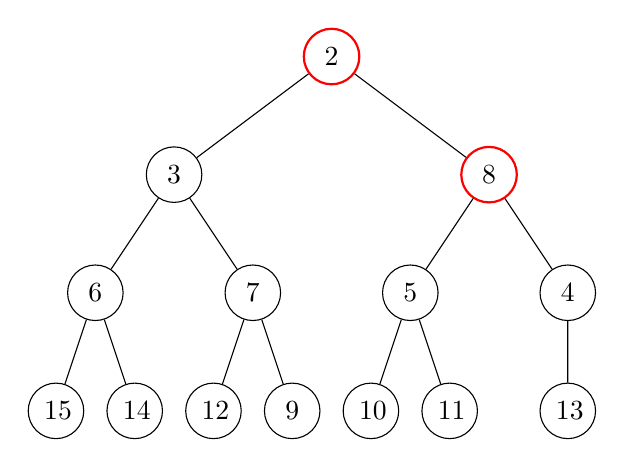
\begin{tikzpicture}[every node/.style={circle, draw=black, text width=0.3cm, align=center},
				   level 1/.style={sibling distance=40mm},
				   level 2/.style={sibling distance=20mm},
				   level 3/.style={sibling distance=10mm}]
\node[draw=red, thick]{2}
	child {node {3}
		child {node {6}
			child {node {15}}
			child {node {14}}
		}
		child {node {7}
			child {node {12}}
			child {node {9}}
		}
	}
	child {node[draw=red, thick] {8}
		child {node {5}
			child {node {10}}
			child {node {11}}
		}
		child {node {4}
			child {node {13}}
		}
	}
;
\end{tikzpicture}
}
\end{minipage}
\begin{minipage}{0.5\textwidth}
\scalebox{0.8}{
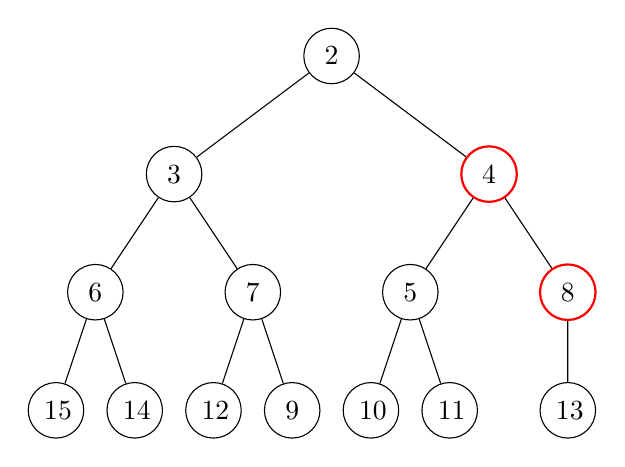
\begin{tikzpicture}[every node/.style={circle, draw=black, text width=0.3cm, align=center},
				   level 1/.style={sibling distance=40mm},
				   level 2/.style={sibling distance=20mm},
				   level 3/.style={sibling distance=10mm}]
\node{2}
	child {node {3}
		child {node {6}
			child {node {15}}
			child {node {14}}
		}
		child {node {7}
			child {node {12}}
			child {node {9}}
		}
	}
	child {node[draw=red, thick] {4}
		child {node {5}
			child {node {10}}
			child {node {11}}
		}
		child {node[draw=red, thick] {8}
			child {node {13}}
		}
	}
;
\end{tikzpicture}
}
\end{minipage}


\section{Grafer}
\subsection{Topologisk sortering}
\subsection{Dijkstra}
\subsection{Prim}
\subsection{Kruskal}
\subsection{Dybde-først}

\section{Kombinatorisk søk}
\section{Rekursjon}

\section{Tekstalgoritmer}

















\newpage

\listoftables
\listoffigures

\end {document}